\documentclass[preprint]{sigplanconf}

% The following \documentclass options may be useful:
%
% 10pt          To set in 10-point type instead of 9-point.
% 11pt          To set in 11-point type instead of 9-point.
% authoryear    To obtain author/year citation style instead of numeric.

\newcommand{\MM}[1]{{\color{blue} TODO(MM): #1}}

\usepackage{amsmath,amsfonts}
\usepackage{mathcomp,amssymb}
\usepackage{dmnatbib}
\usepackage[mathscr]{euscript}
\usepackage{algorithmic,algorithm}

\usepackage{listings}
\lstset{language=C,mathescape=true,numbers=left} % basicstyle={\rm\fontfamily{ppl}\selectfont} trop reconnaissable

\usepackage{tikz}
\usetikzlibrary{arrows,automata}

\tikzstyle{state}=[circle,fill=black!25,minimum size=13pt,inner sep=0pt]
\tikzstyle{rstate}=[rectangle,fill=black!25,minimum size=13pt,inner sep=0pt]
\tikzstyle{transition}=[rectangle,semithick,draw=black!75,
  			  minimum size=4mm]
\tikzstyle{transition2}=[transition,rectangle,thick,dashed,
  			  minimum size=4mm]
\tikzstyle{PRstate}=[circle,double,draw,fill=blue!15,minimum size=13pt,inner sep=0pt]
\tikzstyle{polyhedra}=[blue!25,opacity=0.5,pattern=north west lines,pattern
color=blue]
\tikzstyle{line}=[black,thick]

\usepackage{hyperref}

\newcommand{\abstr}[1]{#1^\sharp}
\newcommand{\parts}[1]{\mathscr{P}(#1)}
\newcommand{\ZZ}{\mathbb{Z}}
\newcommand{\QQ}{\mathbb{Q}}
\newcommand{\RR}{\mathbb{R}}
\newcommand{\widening}{\mathop{\triangledown}}

\begin{document}

\conferenceinfo{PLDI '12}{11-16 June 2012, Beijing} 
\copyrightyear{2012} 
\copyrightdata{[to be supplied]} 

\titlebanner{banner above paper title}        % These are ignored unless
\preprintfooter{short description of paper}   % 'preprint' option specified.

\title{Implicit yaddayadda}
\subtitle{Subtitle Text, if any}

\authorinfo{Anonymous}
           {anonymous}
           {anonymous.gal@gmail.com}

\maketitle

\begin{abstract}
This is the text of the abstract.
\end{abstract}

% \category{CR-number}{subcategory}{third-level}
\category{D.2.4}{Software/Program Verification}{Formal methods}
\category{F.3.1}{Specifying and Verifying and Reasoning about Programs}{Assertions, Invariants, Mechanical verification, Pre- and post-conditions}
\category{F.3.2}{Semantics of Programming Languages}{Program analysis}
\category{F.4.1}{Mathematical Logic}{Logic and constraint programming, Mechanical theorem proving}
\category{I.2.3}{Deduction and Theorem Proving}{Inference engines, Logic programming, Resolution}

\terms
theory, verification, algorithms

\keywords
SMT-solving, static analysis, abstract interpretation, disjunctions

\section{Introduction}
% TODO expliquer 'implicite'
Static analysis by abstract interpretation is a fully automatic program analysis method. When applied to imperative programs, it computes an inductive invariant mapping each program location (or a subset thereof) to a set of states represented symbolically~\cite{CousotCousot_JLC92}.
For instance, if we are only interested in scalar numerical program variables, such a set may be a convex polyhedron (the set of solutions of a system of linear inequalities)~\cite{CousotHalbwachs78,PPL,BagnaraHZ08SCP}.

In such an analysis, information may flow forward (one computes the polyhedron after a program statement as the image, or a super-set thereof, of the polyhedron before by the semantics of the statement) or backward;
forward program analysis computes super-sets of the states reachable from the initialization of the program, backward program analysis computes super-sets of the states co-reachable from some property of interest (for instance, the violation of an assertion).
In forward analysis, control-flow joins correspond to computation of convex hulls if using convex polyhedra (more generally, they correspond to least upper bounds in a lattice); in backward analysis, it is control-flow splits.

It is a known limitation of program analysis by abstract interpretation that this convex hull, or more generally, least upper bound operation, may introduce states that cannot occur in the real program: for instance, the convex hull of the intervals $[-2,-1]$ and $[1,2]$ is $[-2,2]$, strictly larger than the union of the two.
Such introduction may prevent proving desired program properties, for instance $\neq 0$. The alternative is to keep the union symbolic (e.g. compute using $[-2,-1] \cup [1,2]$) and thus compute in the \emph{disjunctive completion}
of the lattice, but the number of terms in the union may grow exponentially with the number of successive tests in the program to analyze, not to mention difficulties for designing suitable widening operators for enforcing the convergence of fixpoint iterations~\cite{PPL,BagnaraHZ08SCP,DBLP:journals/sttt/BagnaraHZ07}.
The exponential growth of the number of terms in the union may be controlled by heuristics that judiciously apply least upper bound operations, as in the \emph{trace partitioning domain} \cite{Rival_Mauborgne_TOPLAS07} implemented in the Astr\'ee analyzer~\cite{ASTREE_TASE07,ASTREE_ESOP05,ASTREE_PLDI03}. % TODO ne garder que les papiers les plus significatifs par rapport au sujet évoqué

Assuming we are  interested in a loop-free program fragment, the above approach of keeping symbolic unions gives the same results as performing the analysis separately over every path in the fragment.
A recent method for finding inductive loop invariants \cite{DBLP:conf/pldi/GulwaniZ10} is based on this idea: each path inside the loop body is considered separately.
Two recent proposals use SMT-solving \cite{Kroening_Strichman_08} as a decision procedure for the satisfiability of first-order arithmetic formulas in order to enumerate only paths that are needed for the progress of the analysis \cite{Gawlitza_Monniaux_ESOP11,Monniaux_Gonnord_SAS11}.

An additional claim of the methods that distinguish paths inside the loop body \cite{DBLP:conf/pldi/GulwaniZ10,Monniaux_Gonnord_SAS11} is that they tend to generate better invariants that methods that do not, by behaving better with respect to the \emph{widening operators} \cite{CousotCousot_JLC92}
used for enforcing convergence when searching for loop invariants by Kleene iterations. A related technique, \emph{guided static analysis} \cite{DBLP:conf/sas/GopanR07}, computes successive loop invariants for increasing subsets of the transitions taken into account, until all transitions are considered; again, the claim is that this approach avoids some gross over-approximation introduced by widenings.

All these methods improve the precision of the analysis by keeping the same abstract domain (say, convex polyhedra) but changing the operations applied and their ordering. An alternative is to change the abstract domain, for instance by moving from intervals to octagons or convex polyhedra \cite{DBLP:journals/lisp/Mine06,Mine_PhD}, or the widening operator: for instance one may replace the classical widening on convex polyhedra \cite{CousotHalbwachs78,Halbwachs_PhD} by an improved version \cite{BagnaraHRZ05SCP}, or use widening ``up to'', that is, use linear inequalities syntactically present in the program source code as possible widening steps~\cite{Polka:FMSD:97}.

There are many possible combinations of the above techniques, and it is not evident which ones perform more or less precisely or more or less efficiency on real-life examples. One needs to experiment. Unfortunately, the published literature on the subject lacks experimental comparative assessments. One purpose of this article is therefore to propose such experimental results.
\medskip

This article makes the following contributions:
\begin{enumerate}
\item We recast the guided static analysis technique from \citet{DBLP:conf/sas/GopanR07} on the expanded multigraph from \citet{Monniaux_Gonnord_SAS11}, considering entire paths instead of individual transitions, using SMT queries and binary decision diagrams.\label{contr:guided_multigraph} (See \S\ref{contr:guided_multigraph})
\item We improve the technique for obtaining disjunctive invariants from \citet{DBLP:conf/pldi/GulwaniZ10} by replacing the explicit exhaustive enumeration of paths by a sequence of SMT queries.\label{contr:disjunctive} (See \S\ref{contr:disjunctive})
\item We implemented these techniques, in addition to ``classical'' iterations and the original guided static analysis, inside a prototype static analyzer.
This tool uses the LLVM bitcode format \cite{Lattner:2004:LCF:977395.977673,LLVM_langref} as input, which can be produced by compilation from C, C++ and Fortran, enabling it to be run on many real-life programs.
With respect to abstract domains on numerical variables, it uses the APRON library \cite{DBLP:conf/cav/JeannetM09}, which supports a variety of abstract domains from which we can choose with minimal changes to our analyzer.
\item We conducted extensive experiments with this tool, on real-life programs, thus obtaining experimental comparisons between the various combinations of techniques. (\S\ref{sec:experiments})
\end{enumerate}

\section{Bases}
\subsection{Static analysis by abstract interpretation}
Let $X$ be the set of possible states of the program variables; for instance, if the program has 3 unbounded integer variables, then $X = \ZZ^3$. The set $\parts{X}$ of subsets of $X$, partially ordered by inclusion, is often referred to as the \emph{concrete domain}. An \emph{abstract domain} is a set $\abstr{X}$ equipped with a partial order $\sqsubseteq$; for instance, it can be the domain of convex polyhedra in $\QQ^3$ ordered by geometric inclusion. In this article, all abstract domains are supposed to contain machine-representable objects, and all $\sqsubseteq$ order relations are supposed to be decidable.
The concrete and abstract domains are connected by a monotone \emph{concretization} function $\gamma: \left(\abstr{X},\sqsubseteq\right) \rightarrow (\parts{X},\subseteq)$: an element $\abstr{x} \in \abstr{X}$ represents a set $\gamma(\abstr{x})$.%
%
\footnote{%
Some presentations of abstract interpretation identify an element $\abstr{x}$ with the set of states $\gamma(\abstr{x})$ that it represents. This leads to simpler notations, but may also confuse if, as in some of our constructions, there exist several $\abstr{x}$ with identical $\gamma(\abstr{x})$, but distinct algorithmic behaviors.}

We also assume a join operator $\sqcap: \abstr{X} \times \abstr{X} \rightarrow \abstr{X}$, with infix notation; in practice, it is generally a least upper bound operation, but we only need it to satisfy $\gamma(\abstr{x}) \cup \gamma(\abstr{y}) \subseteq \gamma(\abstr{x} \sqcap \abstr{y})$ for all $\abstr{x},\abstr{y}$.

\subsection{SMT-solving}
Boolean satisfiability (SAT) is the canonical NP-complete problem: given a propositional formula (e.g. $(a \lor \neg b) \land (\neg a \lor b \lor \neg c)$), decide whether it is satisfiable --- and, if so, output a satisfying assignment.
Despite an exponential worst-case complexity, the DPLL algorithm \cite{Kroening_Strichman_08,Handbook_SAT} solves many useful SAT problems in practice.

SAT was extended to \emph{satisfiability modulo theory} (SMT): in addition to propositional literals, SMT formulas admit atoms from a theory.
For instance, the theories of linear integer arithmetic (LIA) and linear real arithmetic (LRA) have atoms of the form $a_1 x_1 + \dots + a_n x_n \bowtie C$ where $a_1,\dots,a_n,C$ are integer constants, $x_1\,dots,x_n$ are variables (interpreted over $\ZZ$ for LIA and $\RR$ or $\QQ$ for LRA), and $\bowtie$ is a comparison operator $=,\neq,<,\leq,>,\geq$.
Satisfiability for LIA and LRA is NP-complete, yet tools based on DPLL(T) approach \cite{Kroening_Strichman_08,Handbook_SAT} solve many useful SMT problems in practice. All these tools provide a \emph{satisfying assignment} if the problem is satisfiable.

Most SMT solvers, including Z3%
\footnote{\url{http://research.microsoft.com/en-us/um/redmond/projects/z3/}}
Yices,%
\footnote{\url{http://yices.csl.sri.com/}}
and all those supporting the full SMTLIB2 standard \cite{BarST-SMTLIB},
offer an \emph{incremental} interface: the client program specifies the formula as an initially empty conjunction, to which additional constraints are added, and calls a ``check'' function answering whether it is satisfiable; 
it may then backtrack some of the constraints and add other ones without restarting from scratch.

\subsection{A simple, motivating example}
\label{subsec:rate_lim}
Consider the following program, adapted from \cite{Monniaux_Gonnord_SAS11}:
\lstinputlisting{rlim_int.c}
This program implements a construct commonly found in control programs (in e.g. automotive or avionics): a rate limiter. For the sake of simplicity, we chose it to be fed a nondeterministic input clamped between $[-100000,100000]$, but in a real system it would be integrated in a reactive control loop and its input connected to a complex system with unknown output range.

The expected inductive invariant is $\verb|x_old| \in [-100000,100000]$, but classical abstract interpretation using intervals (or octagons or polyhedra) finds $\verb|x_old| \in (-\infty,+\infty)$. % TODO chercher ref Astree
Let us briefly see why.

Widening iterations converge to $\lstinline|x_old| \in (-\infty,+\infty)$; let us now see why decreasing iterations fail to recover the desired invariant. % TODO expliquer widening suivi de narrowing
The \lstinline|x >= x_old+10| test at line~7, if taken, yields $\lstinline|x_old| \in (-\infty,99990)$; followed by \lstinline|x = x_old+10|, we obtain $\lstinline|x| \in (-\infty,100000]$, and the same after union with the no-operation ``else'' branch. Line 8 yields $\lstinline|x| \in (-\infty,+\infty)$.

We could use ``guided widening'' or ``widening with thresholds'', propagating the ``magic values'' $\pm 100000$ associated to \lstinline|x| into~\lstinline|x_old|, but these syntactic approaches cannot directly cope with programs for which $\lstinline|x|  \in [-100000,+100000]$ is itself obtained by analysis.
The guided static analysis of \citet{DBLP:conf/sas/GopanR07} performs slightly better, and obtains $\verb|x_old| \in (-\infty,100000]$.

In contrast, let us distinguish all four possible execution paths through the tests at lines 7 and~8. The path through both ``else'' branches is infeasible; the program is thus equivalent to:
\lstinputlisting{rlim_int2.c}

\begin{figure}
\label{fig:multigraph}
\centering
\begin{minipage}[c]{.19\textwidth}
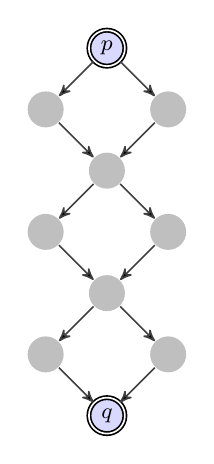
\begin{tikzpicture}[->,>=stealth',auto,node distance=1.1cm,
                    semithick,font=\footnotesize]

	\node[PRstate] (n0) {$p$};
	\node[state] (n1) [below left of=n0] {};
	\node[state] (n2) [below right of=n0] {};
	\node[state] (n3) [below right of=n1] {};
	\node[state] (n4) [below left of=n3] {};
	\node[state] (n5) [below right of=n3] {};
	\node[state] (n6) [below right of=n4] {};
	\node[state] (n7) [below left of=n6] {};
	\node[state] (n8) [below right of=n6] {};
	\node[PRstate] (n9) [below right of=n7] {$q$};

  \path [transition] 
		(n0) edge              node {} (n1);
  \path [transition] 
		(n0) edge              node {} (n2);
  \path [transition] 
		(n1) edge              node {} (n3);
  \path [transition] 
		(n2) edge              node {} (n3);
  \path [transition] 
		(n3) edge              node {} (n4);
  \path [transition] 
		(n3) edge              node {} (n5);
  \path [transition] 
		(n4) edge              node {} (n6);
  \path [transition] 
		(n5) edge              node {} (n6);
  \path [transition] 
		(n6) edge              node {} (n7);
  \path [transition] 
		(n6) edge              node {} (n8);
  \path [transition] 
		(n7) edge              node {} (n9);
  \path [transition] 
		(n8) edge              node {} (n9);
\end{tikzpicture}
\end{minipage} 
$\Longrightarrow$
\begin{minipage}[c]{.19\textwidth}
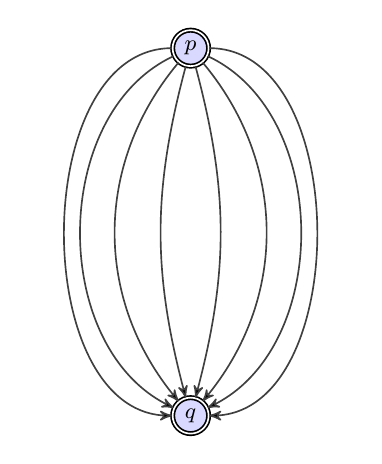
\begin{tikzpicture}[->,>=stealth',auto,node distance=1.1cm,
                    semithick,font=\footnotesize]

	\node[PRstate] (n0) {$p$};
	\node (n1) [below left of=n0] {};
	\node (n2) [below right of=n0] {};
	\node (n3) [below right of=n1] {};
	\node (n4) [below left of=n3] {};
	\node (n5) [below right of=n3] {};
	\node (n6) [below right of=n4] {};
	\node (n7) [below left of=n6] {};
	\node (n8) [below right of=n6] {};
	\node[PRstate] (n9) [below right of=n7] {$q$};

  \path [transition] 
		(n0) edge  [out=0, in=0]            node {} (n9);
  \path [transition] 
		(n0) edge  [out=180, in=180]        node {} (n9);
  \path [transition] 
		(n0) edge  [out=205, in=155]            node {} (n9);
  \path [transition] 
		(n0) edge  [out=230, in=130]            node {} (n9);
  \path [transition] 
		(n0) edge  [out=255, in=105]            node {} (n9);
  \path [transition] 
		(n0) edge  [out=-25, in=25]            node {} (n9);
  \path [transition] 
		(n0) edge  [out=-50, in=50]            node {} (n9);
  \path [transition] 
		(n0) edge  [out=-75, in=75]            node {} (n9);
\end{tikzpicture}
\end{minipage}
\caption{Expansion of the transition graph into a multigraph.}
\end{figure}

Classical interval analysis on this program yields $\lstinline|x_old| \in [-100000,100000]$.
We have transformed the first program into the second, manually pruning out infeasible paths; yet in general the resulting program could be exponentially larger than the first (as in Fig.~\ref{fig:multigraph}), even though not all feasible paths are needed to compute the invariant.
Following recent suggestions \cite{Gawlitza_Monniaux_ESOP11,Monniaux_Gonnord_SAS11}, we avoid this space explosion by keeping the second program implicit while simulating its analysis. This means we work on an implicitly represented transition multigraph (Fig.~\ref{fig:multigraph}); its compact representation is given by the transition graph of the first program.

Contribution \ref{contr:disjunctive} (\S\ref{sec:disjunctive}) replaces the exponential expansion of disjunctive invariant generation from \citet{DBLP:conf/pldi/GulwaniZ10} by an implicit representation;
contribution \ref{contr:guided_multigraph} (\S\ref{sec:guided_multigraph}) recasts the ``guided analysis'' from \citet{DBLP:conf/sas/GopanR07} on an implicit representation of the paths in lieu of the individual transitions.

\subsection{Guided static analysis}
\label{sec:guided}
\emph{Guided static analysis} was proposed by \citet{DBLP:conf/sas/GopanR07} as an improvement over classical upward Kleene iterations with widening.
Consider the following program:
\lstinputlisting{gopan_reps.c}

Classical iterations on the domain of convex polyhedra \cite{Halbwachs_PhD,CousotHalbwachs78} or octagons \cite{Mine_PhD,DBLP:journals/lisp/Mine06} start with $x = 0 \land x = 0$, then continue with $x = y \land 0 \leq x \leq 1$.
The widening operator extrapolates from these two iterations and yields $x = y \land x \geq 0$.
From there, the ``else'' branch at line 5 may be taken; with further widening, $0 \leq y \leq x$ is obtained as a loop invariant, and thus the postcondition computed at line 9 is $x \geq 0 \land y = 0$.
Yet the strongest invariant is $(0 \leq x \leq 51 \land y = x) \lor (51 \leq x \leq 102 \land x+y=102)$, and its convex hull, a convex polyhedron, is
\begin{equation}
y \leq x \land y \leq 102-x \land y \geq 0.\label{eqn:triangle}
\end{equation} % TODO fig
Intuitively, this disappointing result is obtained because widening extrapolates from the first iterations of the loop, but the loop has two different phases ($x \leq 50$ and $x > 50$) with different behaviors, thus the extrapolation from the first phase is not valid for the second.

\citeauthor{DBLP:conf/sas/GopanR07}' idea is to analyze the first phase of the loop with a widening and narrowing sequence, and thus obtain $0 \leq x \leq 50 \land y = x$, and then analyze the second phase, finally obtaining invariant~\ref{eqn:triangle}; each phase is identified by the tests taken or not taken.

The analysis starts by identifying the test taken and not taken during the first iteration of the loop, starting in the loop initialization. The branches not taken are pruned from the loop body, yielding:
\begin{lstlisting}[numbers=none]
  while(1) {
    if(x <= 50) y++;
    else break; /* not taken in phase 1 */
    if(y < 0) break;
    x++;
  }
\end{lstlisting}

Analyzing this loop using widening and narrowing on convex polyhedra or octagons yields the loop invariant $0 \leq x \leq 51 \land y = x$. Now, the transition at line~5 becomes feasible; and we analyze the full loop, starting iterations from $0 \leq x \leq 51 \land y = x$, and obtain invariant~\ref{eqn:triangle}.

More generally, this analysis method considers an ascending sequence of subsets of the transitions in the loop body (left side of Fig.~\ref{fig:multigraph});
for each subset, an inductive invariant is computed for the program restricted to it.
The starting subset are the transitions reachable in one step from the loop initialization.
If for a given subset $S$ in the sequence, no transitions outside of $S$ are reachable from the inductive invariant attached to $S$, then iterations stop;
otherwise, add these transitions to $S$ and iterate more.
Termination ensues from the finiteness of the control-flow graph.


\subsection{Path-focused technique}
\label{sec:path_focusing}

\emph{Path-focused} technique from \citet{Monniaux_Gonnord_SAS11} proposes to
distinguish the different paths in the program in order to avoid loss of
precision due to merge operations. Since the number of paths may be exponential,
the technique keeps them implicit and computes them when needed using
SMT-solving. Then, the iterations are computed over a reduced multigraph instead
of the classical transition graph.

Let $P$ be the set of control points in the transition graph, 
$P_W \subseteq P$ the set of widening points
such that removing the points in $P_W$ gives an acyclic graph.
One can choose a set $P_R$ such that $P_W \subseteq P_R \subseteq P$.

The set of paths is kept implicit by an SMT formula $\rho$ expressing
the semantics of the program, assuming that the transition semantics can be
expressed within a decidable theory. For an easy construction of $\rho$, 
we also assume that the program is expressed in SSA form, meaning that each
variable is only assigned once in the transition graph. This is not a
restriction, since there exist standard algorithms that transform a program into
an SSA format.

This formula contains Boolean \emph{reachability predicates} $b_i$ for each
control points $p_i \notin P_R$, $b_i^s$ and $b_i^d$ for each $p_i \in P_R$, so
that a path 
$p_{i_1} \rightarrow p_{i_2} \rightarrow \dots \rightarrow p_{i_n}$ 
between two points $p_{i_1}, p_{i_n} \in P_R$ 
can easily be expressed as the
cunjunction $b_{i_1}^s \wedge \bigwedge_{2 \leq k < n} b_{i_k} \wedge b_{i_n}^d$.
The Boolean $b_{i}^s$ is $true$ when the path starts at point $p_i$, whereas
$b_i^d$ is $true$ when the path arrives at $p_i$. In other words, we split the
points in $P_R$ into a \emph{source} point, with only outgoing transitions, and
a \emph{destination} point, with only incoming transitions, so that the
resulting graph is acyclic and there is no paths going through control
points in $P_R$.

In order to find focus paths, we solve an SMT formula which is satisfiable when
there exist a path starting at a point $p_i \in P_R$ in a state included in the
actual invariant candidate $X_i$, and arriving at a point $p_j \in P_R$ in a
state outside of $X_j$. In this case, we construct this path using the model and
update $X_j$. When $p_i = p_j$, meaning that the path is actually a self-loop,
we can apply a widening/narrowing sequence, or even compute the transitive
closure of the loop using abstract acceleration. % TODO citation laure gonnord

\section{Guided analysis over the paths}
\label{sec:guided_multigraph}

Guided static analysis \cite{DBLP:conf/sas/GopanR07} applies to the transition
graph of the program. We now present a new technique applying this analysis on the implicit
multigraph from \cite{Monniaux_Gonnord_SAS11}, thus avoiding control flow merges with
unfeasible paths.
In this section, we use the same notations as \ref{sec:path_focusing}, except
that we call the abstract values $X_i^s$ instead of $X_i$ to leave room for
another abstract value $X_i^d$ later in the algorithm.


The combination of these two techniques aims at first discovering a precise
inductive invariant for a subset of paths between two points in $P_R$, 
by the mean of ascending and narrowing iterations. When an
inductive invariant has been found, we add new feasible paths to the subset and
compute an inductive invariant for this new subset, starting with the results
from the previous analysis.
In other words, our technique considers an ascending sequence of
subsets of the paths between two points in $P_R$.
We iterate the operations until we consider the whole program, i.e all the
feasible paths. The result will then be an inductive invariant of the entire program.

\begin{algorithm}
  \begin{algorithmic}
    \STATE \textit{Subset} $\gets \emptyset$
    \WHILE{true}
    \STATE Ascending iteration on \textit{Subset} (lines~\ref{alg=start-ascending}-\ref{alg=end-ascending} in algorithm~\ref{algo:combined})
    \STATE Narrow (line~\ref{alg=narrowing} in algorithm~\ref{algo:combined})
    \STATE Add new paths to \textit{Subset} (lines~\ref{alg=start-add-paths}-\ref{alg=end-add-paths} in algorithm~\ref{algo:combined})
    \ENDWHILE
  \end{algorithmic}
\end{algorithm}


%\MM{Je trouve qu'il manque une vue de haut niveau quelque part par
%  ici. Dire qu'en gros, l'algo, c'est (en pseudo-code ou en langue naturelle) :
%
%Sans ca, enchainer tout de suite sur ``ascending iterations'' est un peu brutal.
%
%Ensuite, on peut rafiner la définition de ``Subset'' ($A$ et $P$), et
%enchainer sur l'algo 2.
%}

\subsection{Algorithm}

The algorithm for Guided static analysis on the implicit multigraph is described
in Algorithm \ref{algo:combined}.

The current working subset of paths, noted $P$, is stored using a
compact representation, such as binary decision diagrams.
We also maintain a set of active control points $A$, containing the points in $P_R$
that still need to be processed. Each time the abstract value of a control point
$p$ is updated, $p$ is inserted in $A$.

We apply the Path-focused technique\cite{Monniaux_Gonnord_SAS11} to
the elements of $A$ until $A$ is empty. 
We also check which paths become feasible, so that we can include them into the
next subset of paths at the next iteration. These new feasible paths are
temporarily stored in a set $P'$. 
When $A$ is empty, it means the
invariant computation of the subgraph is finished. As proposed by
\citet{DBLP:conf/sas/GopanR07}, we can do some narrowing iterations.
These narrowing iterations allow to recover precision lost by
widening, before taking into account new feasible paths.
Thus, our technique combines both the advantages of \emph{Guided Static
Analysis} and \emph{Path-focusing}.
We then restart the analysis with a new subgraph if needed, by adding into $P$
the paths in $P'$. The set of active points $A$ is assigned to $A'$, which is
the set of control points that are starting points of a new feasible path in
$P'$.

\begin{algorithm}
	\caption{Guided static analysis on implicit multigraph}
	\label{algo:combined}
	\begin{algorithmic}[1] 
	\label{alg=combined}

\STATE $A \gets \emptyset$ // States to explore
\STATE $P \gets \emptyset$ // Paths in the current subset
\FORALL {$p \in P_R / I_p \neq \emptyset$}
	\STATE $A \gets A \cup p$
        // \MM{Pourquoi pas juste $A \gets \{p | P_R / I_p \neq \emptyset\}$ a la place de tout le forall?}
\ENDFOR

\WHILE{true}
\STATE $A' \gets \emptyset$ // New states to explore

\STATE $P' \gets \emptyset$ // New paths

\WHILE{$A \neq \emptyset$} \label{alg=start-ascending}
	\STATE Select $p_i \in A$
	\STATE $A \gets A \setminus \{p_i\}$
	\STATE // First only consider the paths already seen (in $P$)
	\STATE PathFocusing($p_i$)
	
	\STATE // add new feasible paths into $P'$
	\STATE ComputeNewPaths($p_i$)

\ENDWHILE \label{alg=end-ascending}
\STATE Narrow \label{alg=narrowing}
\IF {$P' = \emptyset$} \label{alg=start-add-paths}
	\STATE \textbf{break}
\ENDIF \label{alg=end-add-paths}
\STATE // Add the new feasible paths to the graph and restart 
\STATE $P \gets P \cup P'$
\STATE $A \gets A'$
\ENDWHILE

\STATE \RETURN $\{X_i^s,\ i \in P_R\}$


	\end{algorithmic}
\end{algorithm}


\subsection{Ascending iterations by Path-focusing}
\label{subsec:ascending}

The algorithm for computing an inductive invariant over a subgraph is the
Path-focused algorithm from \citet{Monniaux_Gonnord_SAS11} with special
treatment for self loops (line~\ref{alg=pf} in algorithm~\ref{algo:combined}).

In order to find which path to focus on, we construct an SMT formula $f(p_i)$, whose
model when satisfiable is a path that starts in $p_i$, goes to a successor $p_j
\in P_R$ of $p_i$, such that the image of $X_{i}^s$ by the path transformation
is not included in the actual $X_{j}^s$.
Intuitively, such a path makes the abstract value $X_{j}^s$ grow, and thus is
an interesting path to focus on. We loop until the formula becomes unsatisfiable,
meaning that the analysis of $p_i$ is finished.

If we note $Succ(i)$ the set of indices $j$ such that $p_j \in P_R$ is a
successor of $p_i$ in the expanded multigraph, and $X_i^s$ the abstract value
associated to $p_i$ :
$$f(p_i) = \rho \wedge b_i^s \wedge 
\displaystyle\bigwedge_{j \in P_R \atop j \neq i} \neg
b_j^s \wedge x \in X_i^s \wedge \displaystyle\bigvee_{j \in Succ(i)} (b_j^d \wedge
x \notin X_j^s)$$

Since we do not work on the entire transition graph but on a subset of it, we
cunjunct the formula $f(p_i)$ with the actual set of working paths,
noted $P$, expressed as a Boolean formula, where the Boolean variables are the
\emph{reachability predicates} of the control points. We can easily construct
this formula from the binary decision diagram using dynamic programming, and
avoiding an exponentially sized formula. In other words, we force the SMT solver
to give us a path included in $P$.


\subsection{Adding new paths}
\label{subsec:addingpaths}

Our technique computes the fixpoint iterations on a ascending sequence of
subgraphs, until the complete graph is reached.

When the analysis of a subgraph is finished, meaning that the abstract values
for each control points has converged to an inductive invariant for this subgraph,
the next subgraph to work on has to be computed.

This new subgraph is the union of the paths of the previous one with a set
$P'$ of new paths that become feasible regarding the current abstract values.
$P'$ is progressively constructed during the analysis of the subgraph.

We distinguish two phases when analysing a point $p_i \in P_R$:
\begin{enumerate}
\item We search for paths starting at point $p_i$, such that these paths are in
$P$, i.e are included in the working subgraph. Each time we find a path, we
update the abstract value of the destination point of the path. This is the
phase explained in \ref{subsec:ascending}.
\item  When the previous phase terminates, there is no more paths in
$P$, starting at $p_i$, 
that make the abstract values of the successors grow (otherwise, the SMT
solver would not have answered ``\emph{unsat}''). However, there may
exist such paths in the entire multigraph, that are not in $P$. The second phase
computes these paths and adds them to $P'$ (line~\ref{alg=computeNewPaths} in
algorithm~\ref{algo:combined}). We also use SMT solving to discover
these new paths, but we slightly change the SMT formula given to the SMT solver:
we now simply check for the satisfiability of $f(p_i)$ instead of $f(p_i) \wedge
P$. Since we already know that $f(p_i) \wedge P$ is \emph{unsatisfiable}, all
the paths given by the SMT solver won't be in $P$.
\end{enumerate}

It is not necessary to add into $P'$ all the new feasible paths. We just have
to add them one after another, until no more path can make the invariant grow,
as proposed by Algorithm \ref{algo:computepaths}. For that, we use another
abstract value associated to a control point $p_j$, noted $X_j^d$, which is
distinct from $X_j^s$, and initialized to $X_j^s$.

\begin{algorithm}
	\caption{ComputeNewPaths}
	\label{algo:computepaths}
	\begin{algorithmic}[1] 
	\WHILE{true}
	\STATE $res \gets SmtSolve\left[
	 f'(p_i) 
	\right]$
	\IF {$res = unsat$}
		\STATE \textbf{break}
	\ENDIF
	\STATE Compute the path $e$ from the model
	\STATE Update $X^d_j$
	\STATE $P' \gets P' \cup \{e\}$
	\STATE $A \gets A \cup \{p_i\}$
\ENDWHILE

	\end{algorithmic}
\end{algorithm}

\subsection{Termination}
Termination of this algorihm is guaranteed, because:
\begin{itemize}
\item 
the subset of paths $P$ is
strictly increasing at each loop iteration, and bounded by the finite set of
paths in the entire graph. 
\item the set $P'$ always verifies $P \cap P' = \emptyset$ by construction, 
which guarantees that $P'$
will eventually be empty after a finite number of loop iterations.
\end{itemize}

\subsection{Example}

We revise the rate limiter described in \ref{subsec:rate_lim}. In this example,
\emph{Path-focused} technique works well because all the paths starting at the
loop header are actually self loops. In such a case, the technique performs a
widening/narrowing sequence or accelerates the loop, thus leading to a precise
invariant. However, in real cases, there also exist paths that are not
self loops, where \emph{Path-focusing} only performs a widening. 
This widening may induce unrecoverable loss of precision.

Suppose the main loop of the rate limiter contains a nested loop:
\lstinputlisting{rlim_int_loop.c}

We choose $P_R$ as the set of loop headers of the function, plus the initial
state. In this case, we have three elements in $P_R$.
We also unroll the loop once, in order to distinguish the paths that do not go
through the loop from the others:
\begin{lstlisting}[numbers=none]
if (wait) {
   while (wait()) {}
}
\end{lstlisting}

The main loop in the expanded multigraph has then 24 distinct paths, half of
them being self loops, and the other half going to the header of the nested loop.

Guided static analysis from \citet{DBLP:conf/sas/GopanR07} yields at line 5
$\lstinline|x_old| \in~]-\infty,+\infty[$.
Path-focused technique from \citet{Monniaux_Gonnord_SAS11} performs slightly
better, and finds $\lstinline|x_old| \in~]-\infty,10000]$.
Our combined technique gives us the expected invariant 
$\lstinline|x_old| \in~[-10000,10000]$.

In this example, we see that our technique actually combines best of
\emph{Guided Static Analysis} and \emph{Path Focusing}. Still, we need to unroll
the loop once in order to get precise results. Section \ref{sec:disjunctive}
proposes a new technique that gives precise invariants without needing such
graph transformations.

\section{Disjunctive invariants}
\label{sec:disjunctive}

\citet{DBLP:conf/pldi/GulwaniZ10} propose a technique for computing disjunctive invariants, by
distinguishing all the paths inside a loop. In
this section, we propose to improve this technique by using SMT queries to find
interesting paths, the objective being to avoid an explicit exhaustive
enumeration of an exponential number of paths.

This technique is aimed at computing for a loop header $p_i$ a disjunctive invariant
$\bigvee_{1\leq j \leq m} X_{i,j}$. 
To do so, one chooses an integer $\delta \in [1,m]$, and
a mapping function $\sigma: [1,m] \times [1,n] \mapsto [1,m]$, assuming there
are $n$ distinct paths in the loop.  For each
abstract value of the disjunctive invariant, and for each path $\tau_{i,k}$ in the loop, the
image of $X_{i,j}$ by the path is joined with
$X_{i,\sigma(j,k)}$.
Initially, the $\delta$-th abstract value is assigned to the initial states of
$p_i$, and each other abstract value is assigned to bottom.

$m$, $\delta$ and $\sigma$ can be defined heuristically.
For instance, one could define $\sigma$ so that $\sigma(j,k)$ only depends on the
last transition of the path, or else construct it dynamically during the
analysis.

Our method improves this technique in two ways :
\begin{itemize}
\item Instead of enumerating the whole set of paths, we keep them implicit and
compute them only when needed.
\item At each loop iteration of the algorithm explained in
\cite{DBLP:conf/pldi/GulwaniZ10}, an image by a path and a union of abstract
values are computed for each path and each disjunct. 
Lots of these operations may be useless, in the sense that the resulting
abstract value may not change.
In our approach, we do this only for paths and disjuncts that makes the
resulting abstract value grow.
\end{itemize}

Our improvement consists in a modification of the SMT formula we solve in
\ref{sec:guided_multigraph}.
We introduce in this formula Boolean variables $\{d_j, 1 \leq j \leq m\}$, so
that we can easily find in the model which abstract value of the disjunction has
to be chosen to make the invariant grow.
The resulting formula that is given to the SMT solver is defined
by $g(p_i)$.
When the formula is satisfiable, we know that the index $j$ of the starting
disjunct that has to be chosen is the one for which the associate Boolean value
$d_j$ is \emph{true} in the model. Then, we can easily compute the value of 
$\sigma(j,k)$, thus know the index of the disjunct to join with.

\begin{eqnarray*}
g(p_i) = & \rho \wedge b_i^s \wedge 
\displaystyle\bigwedge_{j \in P_R \atop j \neq i} \neg b_j^s  \\
 & \wedge 
\displaystyle\bigvee_{1 \leq k \leq m} (d_k \wedge x \in X_{i,k} \wedge \bigwedge_{l \neq k}
\neg d_l) \\
 & \wedge
\displaystyle\bigvee_{j \in Succ(i)} 
(b_j^d \wedge \bigwedge_{1 \leq k \leq m} (x \notin X_{j,k}))
\end{eqnarray*}

In our algorithm, the initialization of the abstract values slightly differs from
algorithm \ref{algo:combined} line~\ref{alg=X-init}, since we now have to
initialize each disjunct. Line~\ref{alg=X-init} is then replaced by:
\begin{algorithm}[!h]
\begin{algorithmic}[1] 
\FORALL {$k \in \{1,..,m\} \setminus \{\delta\}$}
	\STATE $X_{i,k} \gets \perp$
\ENDFOR
\STATE $X_{i,\delta} \gets I_{p_i}$
\end{algorithmic}
\end{algorithm}

Furthermore, the Path-focused algorithm (line~\ref{alg=pf} from algorithm
\ref{algo:combined}) is enhanced to deal with disjunctive invariants, and
is detailed in algorithm \ref{algo:disjunctive}.

The \emph{Update} function can classically assign to $X_{i,\sigma(j,k)}$ the
value $X_{i,\sigma(j,k)} \widening (X_{i,\sigma(j,k)} \sqcup
\tau_{i,k}(X_{i,j}))$, or can integrate the special treatment for self loops
proposed by \citet{Monniaux_Gonnord_SAS11}, with widening/narrowing sequence or
acceleration.

\begin{algorithm}[!h]
\caption{Disjunctive invariant computation with implicit paths}\label{gulwani2}
\label{algo:disjunctive}
\begin{algorithmic}[1] 
\WHILE {true}
		\STATE $res \gets SmtSolve\left[g(p_i)\right]$
	\IF {$res = unsat$}
		\STATE \textbf{break}
	\ENDIF
	\STATE Compute the path $\tau_{i,k}$ from $res$ 
	\STATE Take $j \in \{ l | d_l = true\}$ 
	\STATE Update($X_{i,\sigma(j,k)})$
\ENDWHILE
\end{algorithmic}
\end{algorithm}

The $\sigma$ function takes as parameters the index of the starting abstract
value, and the path we focus on. If we dynamically construct this function
during the analysis, we should store the results of the sigma function into a
compact representation, such as Algebraic Decision Diagrams.

\section{Experimental comparisons}
\label{sec:experiments}

Our analyzer uses Yices \cite{DBLP:conf/cav/DutertreM06}
 or Microsoft Z3\cite{DBLP:conf/tacas/MouraB08} as SMT-solver.
\section{Conclusion}

% Cas a probleme:
% Initialisation (x,y) à {(1,0), (0,1)}
% puis boucle: si y = 0 alors x++
% fait un polyèdre qui finit par perdre y <= 1 et x >= 0

%\appendix
%\section{Appendix Title}

%This is the text of the appendix, if you need one.

%\acks

% Acknowledgments, if needed.

% We recommend abbrvnat bibliography style.

\bibliographystyle{dmabbrvnat}
\bibliography{implicitization}
\end{document}

% Pour Emacs:
% Local Variables:
% reftex-cite-format: natbib
% End:
